\documentclass[8pt,aspectratio=169]{beamer}
\usetheme{Madrid}
\usepackage{graphicx,booktabs,adjustbox,multicol,amsmath,amssymb,listings,xcolor}
\definecolor{mlblue}{RGB}{0,102,204}
\definecolor{mlpurple}{RGB}{51,51,178}
\definecolor{mllavender}{RGB}{173,173,224}
\definecolor{mllavender2}{RGB}{193,193,232}
\definecolor{mllavender3}{RGB}{204,204,235}
\definecolor{mllavender4}{RGB}{214,214,239}
\definecolor{mlorange}{RGB}{255,127,14}
\definecolor{mlgreen}{RGB}{44,160,44}
\definecolor{mlred}{RGB}{214,39,40}
\definecolor{mlgray}{RGB}{127,127,127}
\definecolor{solkeyword}{RGB}{0,102,153}
\setbeamercolor{palette primary}{bg=mllavender3,fg=mlpurple}
\setbeamercolor{palette secondary}{bg=mllavender2,fg=mlpurple}
\setbeamercolor{palette tertiary}{bg=mllavender,fg=white}
\setbeamercolor{palette quaternary}{bg=mlpurple,fg=white}
\setbeamercolor{structure}{fg=mlpurple}
\setbeamercolor{title}{fg=mlpurple}
\setbeamercolor{frametitle}{fg=mlpurple,bg=mllavender3}
\setbeamercolor{block title}{bg=mllavender2,fg=mlpurple}
\setbeamercolor{block body}{bg=mllavender4,fg=black}
\setbeamertemplate{navigation symbols}{}
\setbeamertemplate{itemize items}[circle]
\setbeamersize{text margin left=5mm,text margin right=5mm}
\newcommand{\bottomnote}[1]{\vfill\vspace{-2mm}\textcolor{mllavender2}{\rule{\textwidth}{0.4pt}}\vspace{1mm}\footnotesize\textbf{#1}}
\usepackage{tikz,pgfplots}
\pgfplotsset{compat=1.18}
\usetikzlibrary{arrows.meta,positioning,shapes.geometric,calc}
\title{Crypto Trading \& Markets: Course Preview}
\subtitle{INTRO Preview}
\author{Prof.~Dr.~Joerg Osterrieder}
\institute{University Lecture Series}
\date{\today}
\begin{document}

% Frame 1: Title
\begin{frame}
\titlepage
\end{frame}

% Frame 2: Why Crypto Trading & Markets Matter
\begin{frame}{Why Crypto Trading \& Markets Matter}
\begin{columns}[T]
\begin{column}{0.62\textwidth}
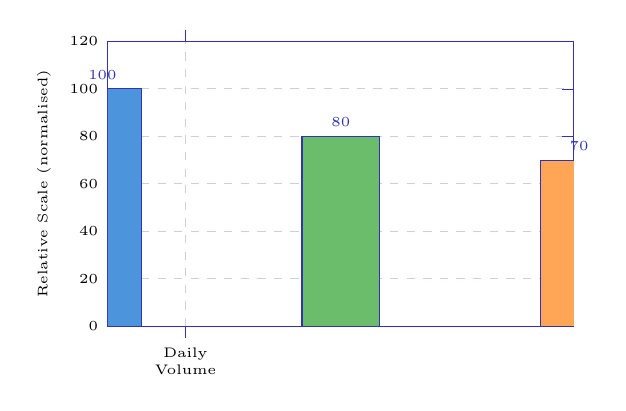
\begin{tikzpicture}
\begin{axis}[
  ybar,
  bar width=28pt,
  width=7.5cm,
  height=5.2cm,
  symbolic x coords={Daily Volume, Exchanges, Algo Trading},
  xtick=data,
  xticklabels={Daily\\Volume, Exchange\\Count, Algo\\Trading Share},
  xticklabel style={font=\tiny, text width=2.5cm, align=center},
  ymin=0, ymax=120,
  ytick={0,20,40,60,80,100,120},
  yticklabel style={font=\tiny},
  ylabel style={font=\tiny},
  ylabel={Relative Scale (normalised)},
  axis line style={draw=mlpurple},
  tick style={draw=mlpurple},
  nodes near coords,
  nodes near coords style={font=\tiny, color=mlpurple},
  point meta=y,
  enlarge x limits=0.25,
  grid=major,
  grid style={dashed, mllavender3},
]
\addplot[fill=mlblue!70,   draw=mlpurple] coordinates {(Daily Volume,   100)};
\addplot[fill=mlgreen!70,  draw=mlpurple] coordinates {(Exchanges,       80)};
\addplot[fill=mlorange!70, draw=mlpurple] coordinates {(Algo Trading,    70)};
\end{axis}
\end{tikzpicture}
\end{column}
\begin{column}{0.36\textwidth}
\vspace{4mm}
\begin{block}{Key Metrics}
\begin{itemize}\setlength\itemsep{4pt}
  \item[\small$\checkmark$] \small \textbf{\$50B+} daily trading volume
  \item[\small$\checkmark$] \small \textbf{500+} active exchanges globally
  \item[\small$\checkmark$] \small \textbf{70\%+} algorithmic trading share
  \item[\small$\checkmark$] \small \textbf{24/7/365} continuous operation
\end{itemize}
\end{block}
\end{column}
\end{columns}
\bottomnote{Crypto markets operate continuously at institutional scale, demanding specialised trading knowledge and tooling.}
\end{frame}

% Frame 3: Trading & Markets Ecosystem at a Glance
\begin{frame}{Trading \& Markets Ecosystem at a Glance}
\vspace{2mm}
\begin{center}
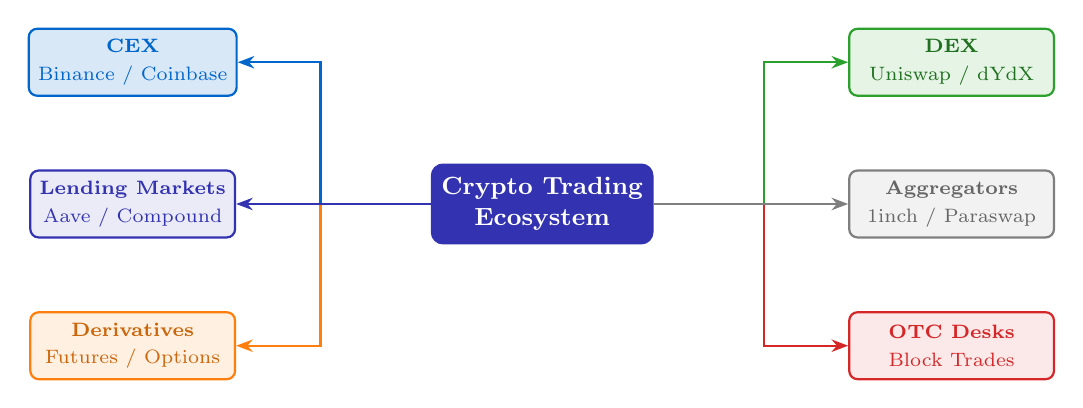
\begin{tikzpicture}[
  cbox/.style={rectangle, rounded corners=4pt, draw=mlpurple, thick,
               fill=mlpurple, minimum width=2.8cm, minimum height=1.0cm,
               font=\small\bfseries, align=center, text=white},
  sbox/.style={rectangle, rounded corners=3pt, thick,
               minimum width=2.6cm, minimum height=0.85cm,
               font=\scriptsize, align=center},
  arr/.style={-{Stealth[length=6pt]}, thick}
]
% Center node
\node[cbox] (center) at (0,0) {Crypto Trading\\Ecosystem};

% Spoke nodes
\node[sbox, draw=mlblue,   fill=mlblue!15,   text=mlblue]              (cex)  at (-5.2, 1.8)
  {\textbf{CEX}\\[2pt]Binance / Coinbase};

\node[sbox, draw=mlgreen,  fill=mlgreen!12,  text=mlgreen!70!black]    (dex)  at ( 5.2, 1.8)
  {\textbf{DEX}\\[2pt]Uniswap / dYdX};

\node[sbox, draw=mlorange, fill=mlorange!12, text=mlorange!80!black]   (deriv) at (-5.2,-1.8)
  {\textbf{Derivatives}\\[2pt]Futures / Options};

\node[sbox, draw=mlred,    fill=mlred!10,    text=mlred]               (otc)  at ( 5.2,-1.8)
  {\textbf{OTC Desks}\\[2pt]Block Trades};

\node[sbox, draw=mlpurple, fill=mlpurple!10, text=mlpurple]            (lend) at (-5.2, 0.0)
  {\textbf{Lending Markets}\\[2pt]Aave / Compound};

\node[sbox, draw=mlgray,   fill=mlgray!10,   text=mlgray!80!black]     (agg)  at ( 5.2, 0.0)
  {\textbf{Aggregators}\\[2pt]1inch / Paraswap};

% Arrows
\draw[arr, draw=mlblue]   (center.west) -- ++(-1.4,0) |- (cex.east);
\draw[arr, draw=mlgreen]  (center.east) -- ++(1.4,0)  |- (dex.west);
\draw[arr, draw=mlorange] (center.west) -- ++(-1.4,0) |- (deriv.east);
\draw[arr, draw=mlred]    (center.east) -- ++(1.4,0)  |- (otc.west);
\draw[arr, draw=mlpurple] (center.west) -- ++(-1.4,0) |- (lend.east);
\draw[arr, draw=mlgray]   (center.east) -- ++(1.4,0)  |- (agg.west);
\end{tikzpicture}
\end{center}
\bottomnote{The ecosystem spans centralised and decentralised venues, derivatives, OTC, lending, and smart aggregation layers.}
\end{frame}

% Frame 4: Market Growth Trajectory
\begin{frame}{Market Growth Trajectory}
\begin{columns}[T]
\begin{column}{0.62\textwidth}
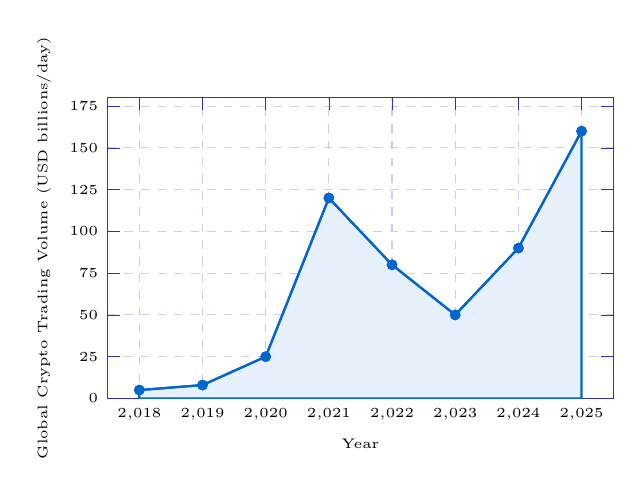
\begin{tikzpicture}
\begin{axis}[
  width=8.0cm,
  height=5.4cm,
  xmin=2017.5, xmax=2025.5,
  ymin=0, ymax=180,
  xtick={2018,2019,2020,2021,2022,2023,2024,2025},
  ytick={0,25,50,75,100,125,150,175},
  xticklabel style={font=\tiny},
  yticklabel style={font=\tiny},
  xlabel style={font=\tiny},
  ylabel style={font=\tiny},
  xlabel={Year},
  ylabel={Global Crypto Trading Volume (USD billions/day)},
  axis line style={draw=mlpurple},
  tick style={draw=mlpurple},
  grid=major,
  grid style={dashed, mllavender3},
]
\addplot[color=mlblue, solid, thick, mark=*, mark size=1.5pt,
         fill=mlblue!10] coordinates {
  (2018,5)(2019,8)(2020,25)(2021,120)(2022,80)(2023,50)(2024,90)(2025,160)
} \closedcycle;
\addplot[color=mlblue, solid, thick, mark=*, mark size=1.5pt] coordinates {
  (2018,5)(2019,8)(2020,25)(2021,120)(2022,80)(2023,50)(2024,90)(2025,160)
};
\end{axis}
\end{tikzpicture}
\end{column}
\begin{column}{0.36\textwidth}
\vspace{4mm}
\begin{block}{Growth Drivers}
\begin{itemize}\setlength\itemsep{4pt}
  \item[\small$\checkmark$] \small \textbf{Institutional entry} via ETFs and custody
  \item[\small$\checkmark$] \small \textbf{DeFi expansion} creating new liquidity pools
  \item[\small$\checkmark$] \small \textbf{Algorithmic strategies} scaling market depth
  \item[\small$\checkmark$] \small \textbf{Regulatory clarity} attracting capital
\end{itemize}
\end{block}
\end{column}
\end{columns}
\bottomnote{Crypto trading volume has grown 30x since 2018, driven by institutional adoption and DeFi innovation.}
\end{frame}

% Frame 5: Course Coverage
\begin{frame}{Course Coverage}
\vspace{2mm}
\begin{center}
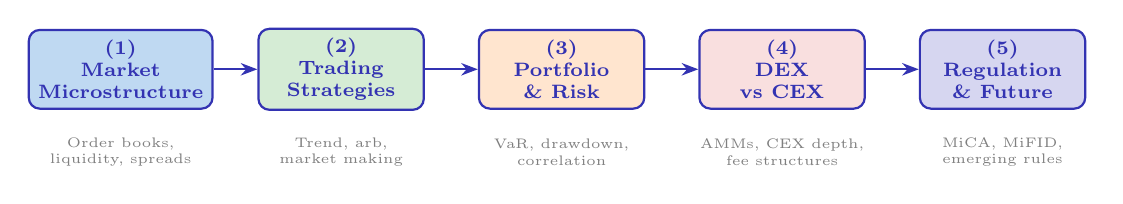
\begin{tikzpicture}[
  procstep/.style={
    rectangle, rounded corners=4pt,
    minimum width=2.1cm, minimum height=1.0cm,
    draw=mlpurple, thick,
    fill=mllavender3,
    font=\scriptsize\bfseries,
    align=center,
    text=mlpurple
  },
  conn/.style={-{Stealth[length=6pt]}, thick, draw=mlpurple}
]
\node[procstep, fill=mlblue!25]    (s1) at (0,0)    {(1)\\Market\\Microstructure};
\node[procstep, fill=mlgreen!20]   (s2) at (2.8,0)  {(2)\\Trading\\Strategies};
\node[procstep, fill=mlorange!20]  (s3) at (5.6,0)  {(3)\\Portfolio\\\& Risk};
\node[procstep, fill=mlred!15]     (s4) at (8.4,0)  {(4)\\DEX\\vs CEX};
\node[procstep, fill=mlpurple!20]  (s5) at (11.2,0) {(5)\\Regulation\\\& Future};

\draw[conn] (s1) -- (s2);
\draw[conn] (s2) -- (s3);
\draw[conn] (s3) -- (s4);
\draw[conn] (s4) -- (s5);

\node[font=\tiny, text=mlgray, align=center, text width=2.1cm] at (0,-1.05)
  {Order books,\\liquidity, spreads};
\node[font=\tiny, text=mlgray, align=center, text width=2.1cm] at (2.8,-1.05)
  {Trend, arb,\\market making};
\node[font=\tiny, text=mlgray, align=center, text width=2.1cm] at (5.6,-1.05)
  {VaR, drawdown,\\correlation};
\node[font=\tiny, text=mlgray, align=center, text width=2.1cm] at (8.4,-1.05)
  {AMMs, CEX depth,\\fee structures};
\node[font=\tiny, text=mlgray, align=center, text width=2.1cm] at (11.2,-1.05)
  {MiCA, MiFID,\\emerging rules};
\end{tikzpicture}
\end{center}
\vspace{4mm}
\begin{columns}[T]
\begin{column}{0.48\textwidth}
\begin{block}{Prerequisites}
\begin{itemize}\setlength\itemsep{2pt}
  \item[\small$\checkmark$] \small Basic blockchain and DeFi knowledge
  \item[\small$\checkmark$] \small Introductory statistics and finance
\end{itemize}
\end{block}
\end{column}
\begin{column}{0.48\textwidth}
\begin{block}{Outcomes}
\begin{itemize}\setlength\itemsep{2pt}
  \item[\small$\checkmark$] \small Design and backtest crypto trading strategies
  \item[\small$\checkmark$] \small Evaluate market structures and regulatory risk
\end{itemize}
\end{block}
\end{column}
\end{columns}
\bottomnote{From microstructure fundamentals to regulatory compliance in five interconnected modules.}
\end{frame}

% Frame 6: What You Will Learn
\begin{frame}{What You Will Learn}
\begin{columns}[T]
\begin{column}{0.44\textwidth}
\vspace{2mm}
\begin{block}{Learning Outcomes}
\begin{itemize}\setlength\itemsep{5pt}
  \item[\small$\checkmark$] \small \textbf{Market microstructure} --- order books, spreads, liquidity dynamics
  \item[\small$\checkmark$] \small \textbf{Trading strategies} --- trend following, arbitrage, market making
  \item[\small$\checkmark$] \small \textbf{Risk management} --- VaR, drawdown limits, portfolio optimisation
  \item[\small$\checkmark$] \small \textbf{Venue comparison} --- CEX depth vs.\ DEX AMMs and hybrid routing
\end{itemize}
\end{block}
\end{column}
\begin{column}{0.54\textwidth}
\vspace{2mm}
\begin{center}
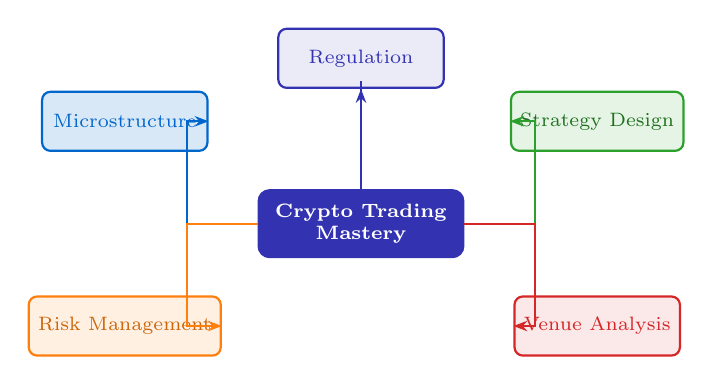
\begin{tikzpicture}[
  cbox/.style={rectangle, rounded corners=4pt, draw=mlpurple, thick,
               fill=mlpurple, minimum width=2.6cm, minimum height=0.85cm,
               font=\scriptsize\bfseries, align=center, text=white},
  fbox/.style={rectangle, rounded corners=3pt, thick,
               minimum width=2.1cm, minimum height=0.75cm,
               font=\scriptsize, align=center},
  farr/.style={-{Stealth[length=5pt]}, thick}
]
% Central node
\node[cbox] (nm) at (0,0) {Crypto Trading\\Mastery};

% Skill nodes
\node[fbox, draw=mlblue,   fill=mlblue!15,   text=mlblue]              (mic)  at (-3.0, 1.3) {Microstructure};
\node[fbox, draw=mlgreen,  fill=mlgreen!12,  text=mlgreen!70!black]    (str)  at ( 3.0, 1.3) {Strategy Design};
\node[fbox, draw=mlorange, fill=mlorange!12, text=mlorange!80!black]   (rsk)  at (-3.0,-1.3) {Risk Management};
\node[fbox, draw=mlred,    fill=mlred!10,    text=mlred]               (reg)  at ( 3.0,-1.3) {Venue Analysis};
\node[fbox, draw=mlpurple, fill=mlpurple!10, text=mlpurple]            (reg2) at ( 0.0, 2.1) {Regulation};

% Arrows
\draw[farr, draw=mlblue]   (nm.west)  -- ++(-0.9,0) |- (mic.east);
\draw[farr, draw=mlgreen]  (nm.east)  -- ++(0.9,0)  |- (str.west);
\draw[farr, draw=mlorange] (nm.west)  -- ++(-0.9,0) |- (rsk.east);
\draw[farr, draw=mlred]    (nm.east)  -- ++(0.9,0)  |- (reg.west);
\draw[farr, draw=mlpurple] (nm.north) -- ++(0,0.6)  |- (reg2.south);
\end{tikzpicture}
\end{center}
\end{column}
\end{columns}
\vspace{1mm}
\bottomnote{By the end you will be able to analyse, design, and evaluate crypto trading systems with professional rigour.}
\end{frame}

\end{document}
